
\chapter{System design}
\section{System overview} \label{sec:system}
Here you insert a block diagram of your voltage regulationa nd signal conditioning system. 
Try to explain \textbf{what} configiation you chose and \textbf{why}. 
There is no need to specify the capacitor and resistor values here, but you want to capture the higher-level functional arrangement you have opted for. The diagram ties together the other chapters in this report and helps the reader understand how you have connected the different funtional blocks together to produce the outputs. For example, a block could be ``Differential amplifier'' or ``level shifting op-amp'' or ``Low-pass filter'' or ``Linear regulator'' and the like. 
Please use a drawing application, such as draw.io, MS Visio, or Power Point and export it as a PDF, so it looks good. If you feel brave, draw them in \LaTeX using Inkscape/\texttt{TikZ}.
Fig.\ \ref{fig:system_diagram} is a bad example that is completely irrelevant and just holds space for your beautiful system diagram. 
\begin{figure}
    \centering
    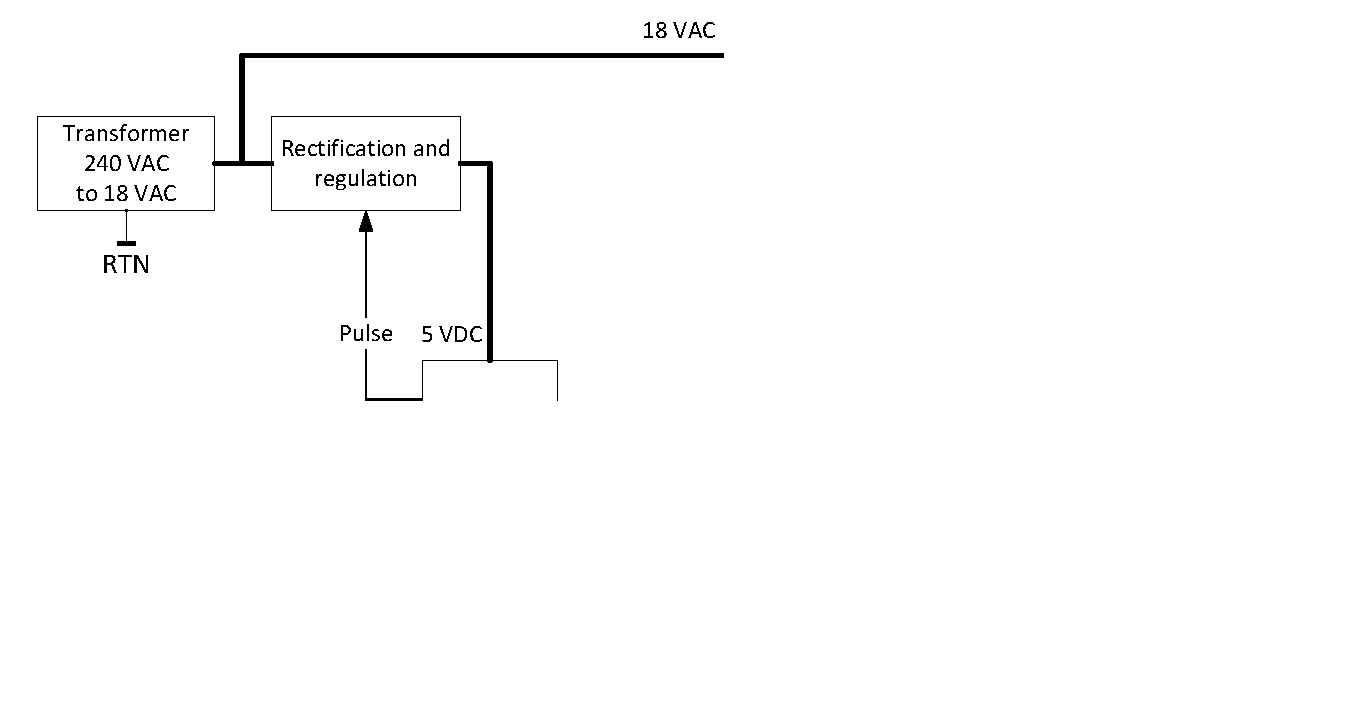
\includegraphics[width = 0.5\linewidth]{Figures/PowerSystemDiagram.pdf}
    \caption{System diagram}
    \label{fig:system_diagram}
\end{figure}

\vfill









